
%------------------------------------------------------------------------------
% 
% Lightning talk on signal transmission
% title:  signal-transmission.tex
% author: Dominik Gedon
% date:   24.01.2020
%
% todo: replace pictures/digrams with self generated ones
%------------------------------------------------------------------------------
\documentclass[ngerman]{beamer}

\usepackage{beamerthemesplit} %// Activate for custom appearance
\usepackage[T1]{fontenc}
\usepackage{inputenc}
\usepackage{graphicx}
\usepackage{svg}
\usepackage{amsmath}
\usepackage[font=small]{caption}
\usepackage{xcolor}
\usepackage{appendixnumberbeamer}
\usepackage{siunitx}
\usepackage{wrapfig}
\usepackage{hyperxmp, hyperref}
\usepackage[
	type={CC},
	modifier={by-sa},
	version={4.0},
	lang={german}
]{doclicense}
\sisetup{
	range-phrase = to,
	per-mode = fraction,
	inter-unit-product = cdot,
	detect-family = false
} 
\usetheme{metropolis}

%------------------------------------------------------------------------------
% definitions 
%------------------------------------------------------------------------------
\newcommand\titlename{Signal transmission }
\graphicspath{./figures/}
\metroset{sectionpage=simple, subsectionpage=none, numbering=fraction}
\setbeamertemplate{frame footer}{\titlename | Dominik Gedon}


%---------------------------------------------------------------------------------------
%---------------------------------------------------------------------------------------
\title[\titlename]{\titlename}
%\subtitle{Nachrichtentechnische Systeme}
\author{Dominik Gedon}
\date{27. Januar 2020}

\begin{document}

% title page
\maketitle

% Table of contents
\begin{frame}[plain]{Inhalt}
	\setbeamertemplate{section in toc}[sections numbered]
	\tableofcontents[hideallsubsections]
\end{frame}


%---------------------------------------------------------------------------------------
\section{Overview}
%---------------------------------------------------------------------------------------
\begin{frame}{Overview}
	\textbf{Mission}
	\begin{itemize}[label={-}, itemsep=2ex]
		\item Transmission of information/messages over
		\begin{itemize}[label={}]
			\item space (from place to place)
			\item time (storage)
		\end{itemize}
		\item in the most efficient way
	\end{itemize} 
	
	\textbf{Fields of application}
	\begin{itemize}[label={-}, itemsep=1ex]
		\item Network (LAN, WLAN, mobile communication)
		\item IT systems (computer, smartphones, etc.)
		\item Storage media (CD, DVD, Blu-ray disk, HDDs)\newline
		$\Longrightarrow$ Almost \textbf{\alert{everywhere}}	
	\end{itemize} 
\end{frame}


\begin{frame}{Signal transmission}
	\begin{figure}[htbp]
 	 	\centering 	
 		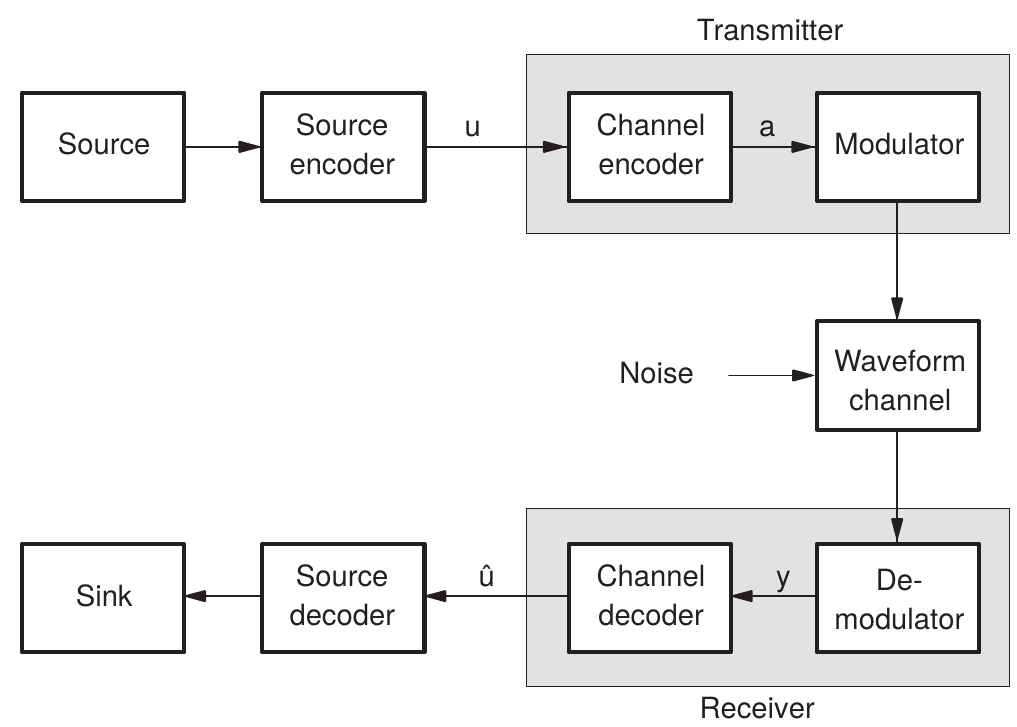
\includegraphics[scale=0.22]{/figures/signal_transmission} 	 
 		\caption {Overview signal transmission \cite{friedrichs}}
	\end{figure}
\end{frame}


\begin{frame}{Signals}
	\textbf{What is a signal?}
	\begin{itemize}[label={-}, itemsep=2ex]
		\item Representation of messages/information by a physical process
		\item e.g. voltage/current versus time, sound pressure over time		
	\end{itemize} 
	\textbf{Types of signals}	
	\begin{itemize}[label={-}, itemsep=2ex]
		\item Analog signals vs. digital signals
		\item Deterministic (known) vs. random (unknown) 
	\end{itemize} 
\end{frame}

\begin{frame}{Source/Transmitter}
	\begin{itemize}[label={-}, itemsep=2ex]
		\item Adaptation of the source signal to the transmission medium
		\item Reduction of redundancy + irrelevance for efficient use of the transmission channel \alert{(source coding)}
		\item Redundancy insertion to secure the message against interference and falsification \alert{(channel coding)}
		\item Efficient use of available transmission power and signal bandwidth
	\end{itemize} 	
\end{frame}


\begin{frame}{Channel}
	\textbf{What is a channel?}
	\begin{itemize}[label={-}, itemsep=2ex]
		\item Wire, air, storage device
		\item Determined by the physical properties of the transmission medium
	\end{itemize} 
	\textbf{What does it do?}
	\begin{itemize}[label={-}, itemsep=2ex]
		\item Carriage of the transmitted signal to the receiver
		\item Channel attenuates the transmit signal, causes distortion
		\item Interruptions (noise, interference) overlap
		\end{itemize} 	
	\end{frame}


\begin{frame}{Sink/Receiver}
	\begin{itemize}[label={-}, itemsep=2ex]
	\item Recovery of the source signal from the received signal
	\item Extraction of as much information as possible about the source signal contained in the received signal
	\item Adaptation of the received signal to sink
	\end{itemize} 
\end{frame}



%\begin{frame}{Modulation}
%\begin{itemize}[label={-}, itemsep=2ex]	
%	\item Generation of a high-frequency transmission signal
%	
%	\end{itemize} 	
%\end{frame}

\begin{frame}{Coding}
\textbf{What is a coding?}

A mapping rule that uniquely assigns a character or string to each character of a source word.

$ \underbrace{\begin{matrix} (a & b & c)\end{matrix}}
_\text{source alphabet} = \underbrace{\begin{matrix} (0 & 1)\end{matrix}}_\text{target alphabet}$\newline\newline
Mapping: $ \begin{matrix} (a \mapsto 0, b \mapsto 01, c \mapsto 011)\end{matrix}$

\textbf{Example}

Source word: acabc\newline
$ \underbrace{\begin{matrix} (acabc)\end{matrix}}
_\text{source word} = \underbrace{\begin{matrix} (0 &011 &0 &01 &011)\end{matrix}}_\text{code word}$

\end{frame}


%---------------------------------------------------------------------------------------
\section{Source coding}
%---------------------------------------------------------------------------------------
\begin{frame}{Recap: Signal transmission}
	\begin{figure}[htbp]
 	 	\centering 	
 		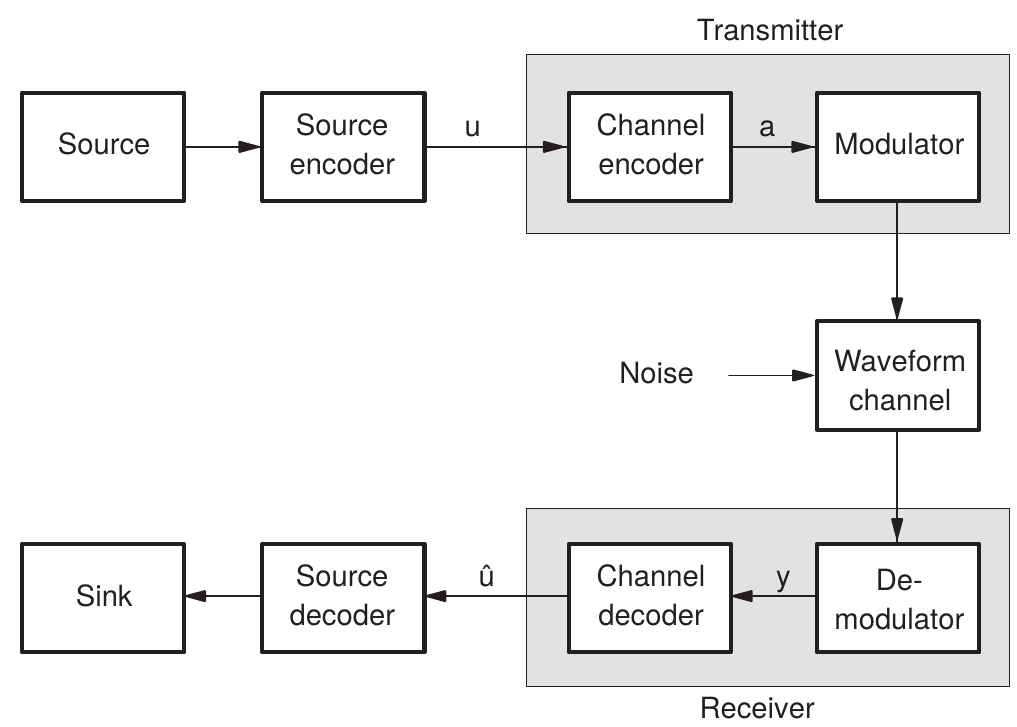
\includegraphics[scale=0.22]{/figures/signal_transmission} 	 
 		\caption {Overview signal transmission \cite{friedrichs}}
	\end{figure}
\end{frame}

\begin{frame}{Source coding}
	\textbf{What is it?}
	\begin{itemize}[label={-}, itemsep=2ex]
		\item Removal of redundant information
		\item Data compression
	\end{itemize} 
	\textbf{How is it achieved?}
	\begin{itemize}[label={-}, itemsep=2ex]
		\item Mapping of source words with high probability to short code words
	\end{itemize} 
\end{frame}


\begin{frame}{Source coding: Example I - Huffman coding}
\textbf{Assumption:}\newline
$Pr\{A\} = 0,8 \newline Pr\{B\} = 0,2$
	\begin{figure}[htbp]
 	 	\centering 	
 		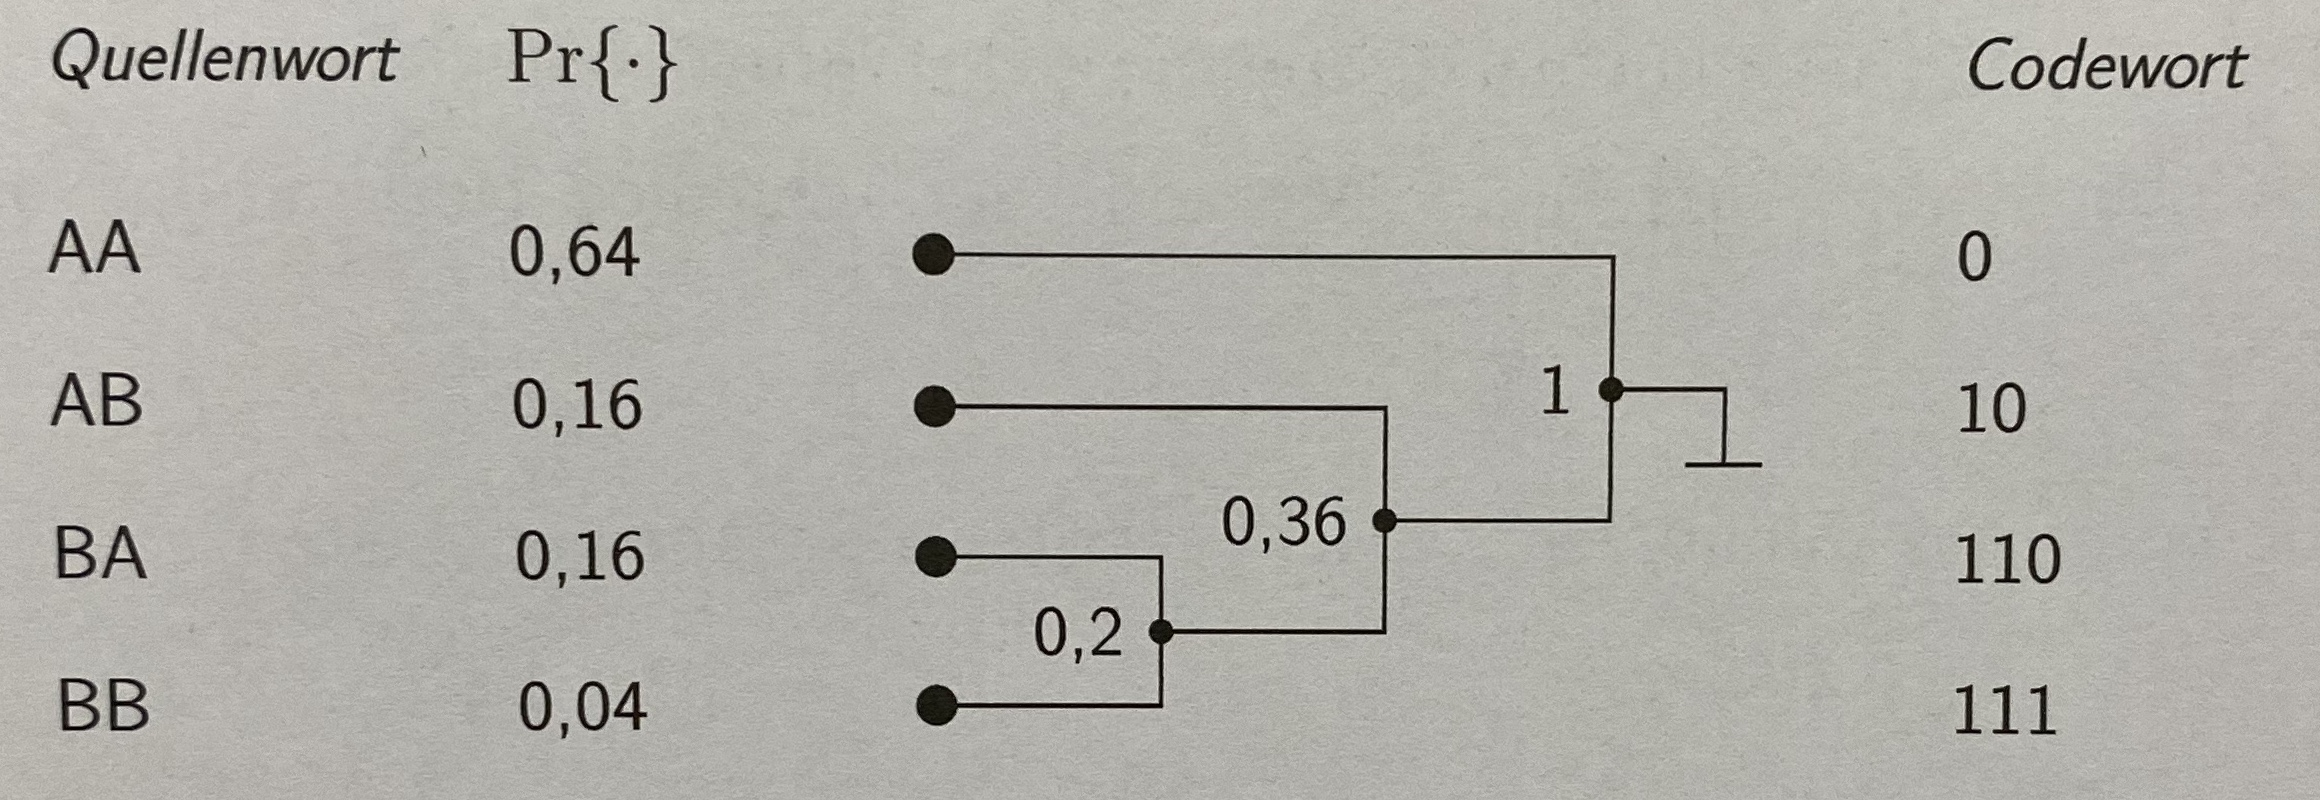
\includegraphics[scale=0.135]{/figures/huffman1} 	 
 		\caption {Example I Huffman coding \cite{huber}}
	\end{figure}
\end{frame}

\begin{frame}{Source coding: Example II - Huffman coding}
	\begin{figure}[htbp]
 	 	\centering 	
 		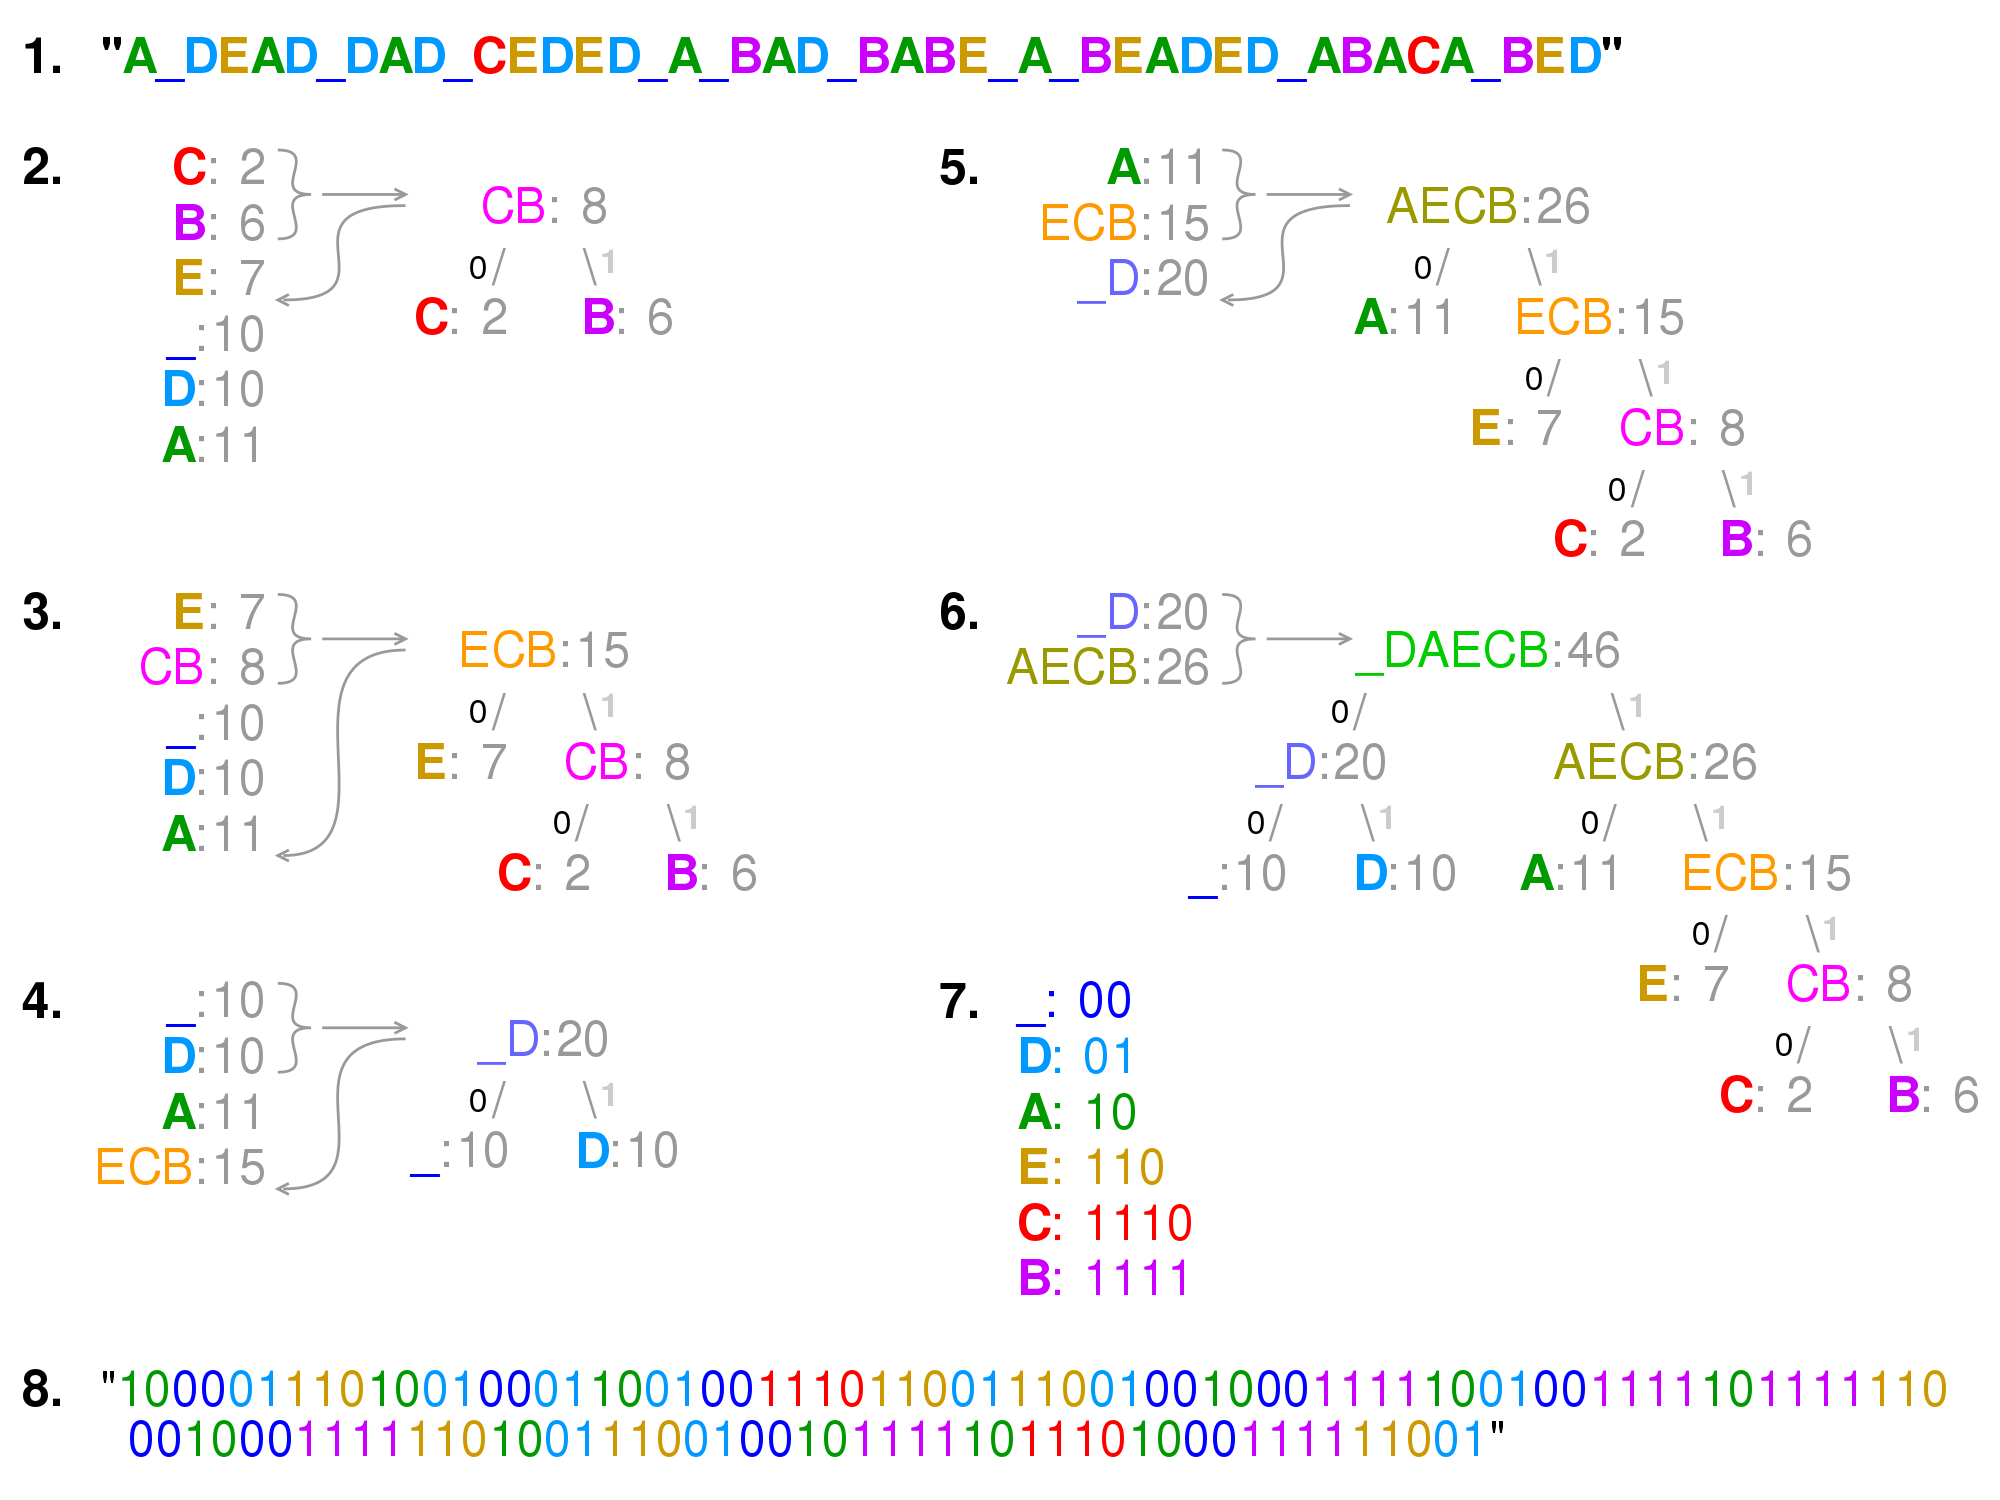
\includegraphics[scale=0.125]{/figures/huffman2} 	 
 		\caption {Example II Huffman coding \cite{huffman}}
	\end{figure}
\end{frame}


%---------------------------------------------------------------------------------------
\section{Channel coding}
%---------------------------------------------------------------------------------------
\begin{frame}{Recap: Signal transmission}
	\begin{figure}[htbp]
 	 	\centering 	
 		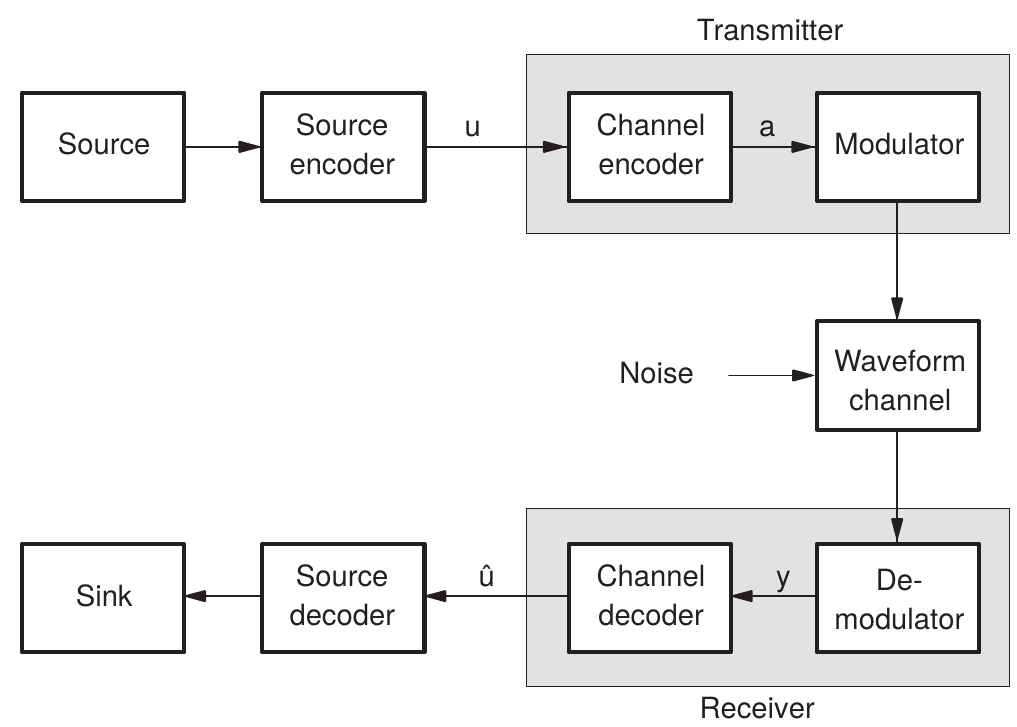
\includegraphics[scale=0.22]{/figures/signal_transmission} 	 
 		\caption {Overview signal transmission \cite{friedrichs}}
	\end{figure}
\end{frame}

\begin{frame}{Channel coding: What is it?}
	\begin{itemize}[label={-}, itemsep=2ex]
		\item When transmitting and storing data, \alert{errors} must be expected
		\item Securing the message against errors\newline
		 $\Longrightarrow$ Adding \textbf{\alert{redundancy}} on the transmitting side
		\item Receiver uses this redundancy to detect + correct errors
		\item \textbf{Task}: \alert{error detection} and if necessary \alert{error correction} based on redundancy	
	\end{itemize}	  
\end{frame}


\begin{frame}{Channel coding: Example}
	\begin{itemize}[label={-}, itemsep=2ex]
		\item International Standard Book Number (\textbf{ISBN})
		\begin{figure}[htbp]
 	 		\centering 	
 			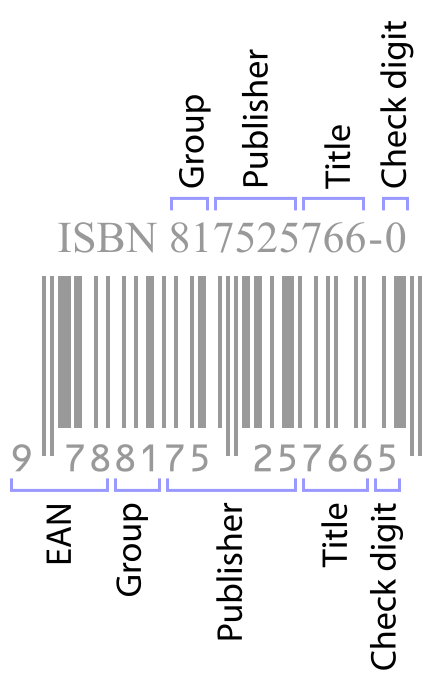
\includegraphics[scale=0.25]{/figures/ISBN} 	 
 			\caption {A 10-digit ISBN and the corresponding EAN‑13 \cite{isbn}}
		\end{figure}
	\end{itemize}
\end{frame}

%---------------------------------------------------------------------------------------
\section{Summary}
%---------------------------------------------------------------------------------------
\begin{frame}{Summary}
	\begin{itemize}[label={-}, itemsep=2ex]
		\item Signal transmission is almost everywhere\newline\newline
		$\Rightarrow$ Processing of the signal is necessary
		\item Data compression (source coding)			
		\item Securing the message against errors (channel coding)\newline
		 $\Rightarrow$ \textbf{\alert{redundancy}}
	\end{itemize}  
\end{frame}


%---------------------------------------------------------------------------------------
\begin{frame}{Source}
%---------------------------------------------------------------------------------------
  Get the source of this presentation from
  \begin{center}\url{github.com/nodeg/talks}\end{center}
  The presentation \emph{itself} is licensed under a  \href{https://creativecommons.org/licenses/by-sa/4.0/}{Attribution-ShareAlike 4.0 International (CC BY-SA 4.0) License}.
  \begin{center}\doclicenseImage\end{center}
\end{frame}

%---------------------------------------------------------------------------------------
\begin{frame}[allowframebreaks]{References}
%---------------------------------------------------------------------------------------
  \bibliography{signal-transmission}
  \bibliographystyle{abbrv}
\end{frame}

\end{document}
